\documentclass{beamer}
\usepackage{graphicx}
\usepackage{ragged2e}
\usepackage{booktabs}
\usepackage{tcolorbox}
\usepackage{amsmath, esint}
\usepackage{tikz}
\usetikzlibrary{backgrounds, positioning, arrows, scopes, shapes, shapes.misc, shapes.multipart}
\tikzset{
    cross/.style={cross out, draw=black, minimum size=2*(#1-\pgflinewidth), inner sep=0pt, outer sep=0pt},
    cross/.default={10pt},
    split/.style={rectangle split, rectangle split parts=7, draw, inner sep=0ex, rectangle split horizontal, minimum size=4ex},
    textstyle/.style={text height=1.5ex, text depth=.25ex}
}

\usepackage[plain]{algorithm}
\usepackage{algorithmic}

\usepackage{xcolor} 
\definecolor{LightGray}{gray}{0.975}

%\usetheme{Warsaw}
\usefonttheme{serif} 

\title[L3 Divide \& Conquer]{Introduction to Algorithms \\ Lecture 3: Divide and Conquer}
\author{Prof. Charles E. Leiserson and Prof. Erik Demaine \\ Massachusetts Institute of Technology}
\date{\today}

\setbeamertemplate{navigation symbols}{}%remove navigation symbols

\defbeamertemplate*{footline}{shadow theme}{%
    \leavevmode%
    \hbox{
        \begin{beamercolorbox}[wd=.5\paperwidth,ht=2.5ex,dp=1.125ex,leftskip=.3cm plus1fil,rightskip=.3cm]{author in head/foot}%
            \usebeamerfont{author in head/foot} Introduction to Algorithms: \hfill \insertshorttitle
        \end{beamercolorbox}%
        \begin{beamercolorbox}[wd=.5\paperwidth,ht=2.5ex,dp=1.125ex,leftskip=.3cm,rightskip=.3cm plus1fil]{title in head/foot}%
            \usebeamerfont{title in head/foot} \hfill \insertframenumber\,/\,\inserttotalframenumber%
        \end{beamercolorbox}
    }%
    \vskip0pt%
}

\AtBeginSection[]{
    \begin{frame}<beamer>
    \frametitle{Plan}
    \tableofcontents[currentsection]
    \end{frame}
}

\newcommand{\toRight}[1]{
    \begin{FlushRight}
        {\small #1}
    \end{FlushRight}
}

\begin{document}

\frame{\titlepage}

\begin{frame}{Introduction to Algorithms}
    \centering
    
\includegraphics[width=0.45\textwidth]{figures/book_cover.jpg} \\
    \vspace{5mm}{
        \tiny
        Content has been extracted from \textit{Introduction to Algorithms}, Fourth Edition, by Cormen, Leiserson, Rivest, and Stein. MIT Press. 2022.\\
        Visit \url{https://mitpress.mit.edu/9780262046305/introduction-to-algorithms/}.\\
        Original slides from \textit{Introduction to Algorithms 6.046J/18.401J}, Fall 2005 Class by Prof. Charles Leiserson and Prof. Erik Demaine. MIT OpenCourseWare Initiative available at \url{https://ocw.mit.edu/courses/6-046j-introduction-to-algorithms-sma-5503-fall-2005/}.\\
    }
\end{frame}

\begin{frame}{The Divide \& Conquer Design Paradigm}
    \begin{enumerate}
        \item \textbf{\Large Divide} the problem (instance) into subproblems.
        \item \textbf{\Large Conquer} the subproblems by solving them recursively.
        \item \textbf{\Large Combine} subproblems solutions.
    \end{enumerate}
\end{frame}

\begin{frame}{Merge-sort}
    \begin{enumerate}
        \item \textbf{\Large Divide:} Trivial.
        \item \textbf{\Large Conquer:} Recursively sort 2 subarrays.
        \item \textbf{\Large Combine:} Linear-time merge.
    \end{enumerate}
\end{frame}

\begin{frame}{Merge-sort}
    \begin{enumerate}
        \item \textbf{\Large Divide:} Trivial.
        \item \textbf{\Large Conquer:} Recursively sort 2 subarrays.
        \item \textbf{\Large Combine:} Linear-time merge.
    \end{enumerate}
    \vspace{4mm}
    $$
        T(n) = 2T\left(\frac{n}{2}\right) + \Theta(n)
    $$ \pause
    \begin{tikzpicture}[remember picture,overlay]
        \draw[red,thick,->]   (2.40, -0.40) to [out=90,in=270](4.85, 0.65);
        \node[] at (2.40, -0.50) {\small Number of subproblems.}; \pause
        \draw[blue,thick,->]  (4.40, -1.30) to [out=90,in=270](5.70, 0.40);
        \node[] at (4.40, -1.50) {\small Subproblem size.}; \pause
        \draw[orange,thick,->](8.40, -0.40) to [out=90,in=270](6.90, 0.55);
        \node[] at (8.40, -0.50) {\small Work dividing and combining.}; \pause
    \end{tikzpicture}
\end{frame}

\begin{frame}{Master Theorem (reprise)}
    \small
    $$
        T(n) = aT\left(\frac{n}{b}\right) + f(n)
    $$ \pause
    \begin{itemize}
        \vspace{-5mm}
        \item[Case 1]
            \begin{align*}
                f(n) = O\left(n^{\log_b a - \varepsilon} \right) \text{, constant }\varepsilon > 0 \\ \implies T(n) = \Theta(n^{log_b a}) \text{.}
            \end{align*} \pause
        \vspace{-5mm}
        \item[Case 2]
            \begin{align*}
                f(n) = \Theta\left(n^{\log_b a}\lg^k n \right) \text{, constant }k \geq 0 \\ \implies T(n) = \Theta(n^{log_b a}\lg^{k + 1} n) \text{.}
            \end{align*} \pause
        \vspace{-5mm}
        \item[Case 3]
            \begin{align*}
                f(n) = \Omega\left(n^{lob_b(a) + \varepsilon} \right) \text{, constant }\varepsilon > 0 \text{, and regularity condition } \\ \implies T(n) = \Theta(f(n)) \text{.}
            \end{align*} \pause
    \end{itemize}
\end{frame}

\begin{frame}{Master Theorem (reprise)}
    \small
    $$
        T(n) = aT\left(\frac{n}{b}\right) + f(n)
    $$
    \begin{itemize}
        \vspace{-5mm}
        \item[Case 1]
            \begin{align*}
                f(n) = O\left(n^{\log_b a - \varepsilon} \right) \text{, constant }\varepsilon > 0 \\ \implies T(n) = \Theta(n^{log_b a}) \text{.}
            \end{align*}
        \vspace{-5mm}
        \item[Case 2]
            \begin{align*}
                f(n) = \Theta\left(n^{\log_b a}\lg^k n \right) \text{, constant }k \geq 0 \\ \implies T(n) = \Theta(n^{log_b a}\lg^{k + 1} n) \text{.}
            \end{align*}
        \vspace{-5mm}
        \item[Case 3]
            \begin{align*}
                f(n) = \Omega\left(n^{lob_b(a) + \varepsilon} \right) \text{, constant }\varepsilon > 0 \text{, and regularity condition } \\ \implies T(n) = \Theta(f(n)) \text{.}
            \end{align*}
    \end{itemize}
    \begin{align*}
        \text{\textsc{Merge-sort:} } a = 2, b = 2 \implies n^{log_b a} = n^{log_2 2} = n \\ \implies \text{ Case 2 } (k = 0) \implies T(n) = \Theta(n \lg n) \text{.}
    \end{align*}
\end{frame}


\section{Binary Search}

\begin{frame}{Binary Search}
    Find an element in a sorted array:
    \begin{enumerate}
        \item \textbf{\Large Divide:} Check middle element.
        \item \textbf{\Large Conquer:} Recursively search 1 subarray.
        \item \textbf{\Large Combine:} Trivial.
    \end{enumerate}
\end{frame}

\begin{frame}[fragile]{Binary Search}
    Find an element in a sorted array:
    \begin{enumerate}
        \item \textbf{\Large Divide:} Check middle element.
        \item \textbf{\Large Conquer:} Recursively search 1 subarray.
        \item \textbf{\Large Combine:} Trivial.
    \end{enumerate}
    \begin{exampleblock}{\small Example:}
        Find 9 \\
        \vspace{5mm}
        \begin{tikzpicture}[remember picture,overlay]
            \node (rect) at (4, 0) [fill=red!20,minimum width=7.05cm,minimum height=0.68cm] {};
            \node[split,text width=6ex] at (4, 0) {
                                \hfil \Large  3\hfil
                \nodepart[]{two}  \hfil \Large  5\hfil
                \nodepart{three}\hfil \Large  7\hfil
                \nodepart{four} \hfil \Large  8\hfil
                \nodepart{five} \hfil \Large  9\hfil
                \nodepart{six}  \hfil \Large 12\hfil
                \nodepart{seven}\hfil \Large 15\hfil
            };
            \pause
            \node (rect) at (4, 0) [fill=red!20,minimum width=7.05cm,minimum height=0.68cm] {};
            \node (rect) at (4, 0) [fill=yellow!20,minimum width=4ex,minimum height=0.68cm] {};
            \node[split,text width=6ex] at (4, 0) {
                                \hfil \Large  3\hfil
                \nodepart[]{two}  \hfil \Large  5\hfil
                \nodepart{three}\hfil \Large  7\hfil
                \nodepart{four} \hfil \Large  8\hfil
                \nodepart{five} \hfil \Large  9\hfil
                \nodepart{six}  \hfil \Large 12\hfil
                \nodepart{seven}\hfil \Large 15\hfil
            };
            \pause
            \node (rect) at (4, 0) [fill=white,minimum width=7.05cm,minimum height=0.68cm] {};
            \node (rect) at (6, 0) [fill=red!20,minimum width=3.025cm,minimum height=0.68cm] {};
            \node[split,text width=6ex] at (4, 0) {
                                \hfil \Large  3\hfil
                \nodepart[]{two}  \hfil \Large  5\hfil
                \nodepart{three}\hfil \Large  7\hfil
                \nodepart{four} \hfil \Large  8\hfil
                \nodepart{five} \hfil \Large  9\hfil
                \nodepart{six}  \hfil \Large 12\hfil
                \nodepart{seven}\hfil \Large 15\hfil
            };
            \pause
            \node (rect) at (6, 0) [fill=red!20,minimum width=3.025cm,minimum height=0.68cm] {};
            \node (rect) at (6, 0) [fill=yellow!20,minimum width=4ex,minimum height=0.68cm] {};
            \node[split,text width=6ex] at (4, 0) {
                                \hfil \Large  3\hfil
                \nodepart[]{two}  \hfil \Large  5\hfil
                \nodepart{three}\hfil \Large  7\hfil
                \nodepart{four} \hfil \Large  8\hfil
                \nodepart{five} \hfil \Large  9\hfil
                \nodepart{six}  \hfil \Large 12\hfil
                \nodepart{seven}\hfil \Large 15\hfil
            };
            \pause
            \node (rect) at (6, 0) [fill=white,minimum width=3.025cm,minimum height=0.68cm] {};
            \node (rect) at (5, 0) [fill=red!20,minimum width=1.012cm,minimum height=0.68cm] {};
            \node[split,text width=6ex] at (4, 0) {
                                \hfil \Large  3\hfil
                \nodepart[]{two}  \hfil \Large  5\hfil
                \nodepart{three}\hfil \Large  7\hfil
                \nodepart{four} \hfil \Large  8\hfil
                \nodepart{five} \hfil \Large  9\hfil
                \nodepart{six}  \hfil \Large 12\hfil
                \nodepart{seven}\hfil \Large 15\hfil
            };
            \pause
            \node (rect) at (5, 0) [fill=red!20,minimum width=1.012cm,minimum height=0.68cm] {};
            \node (rect) at (5, 0) [fill=yellow!20,minimum width=4ex,minimum height=0.68cm] {};
            \node[split,text width=6ex] at (4, 0) {
                                \hfil \Large  3\hfil
                \nodepart[]{two}  \hfil \Large  5\hfil
                \nodepart{three}\hfil \Large  7\hfil
                \nodepart{four} \hfil \Large  8\hfil
                \nodepart{five} \hfil \Large  9\hfil
                \nodepart{six}  \hfil \Large 12\hfil
                \nodepart{seven}\hfil \Large 15\hfil
            };
        \end{tikzpicture}
    \end{exampleblock}
\end{frame}

\begin{frame}{Recurrence for Binary Search}
    $$
        T(n) = 1T\left(\frac{n}{2}\right) + \Theta(1)
    $$ \pause
    \begin{tikzpicture}[remember picture,overlay]
        \draw[red,thick,->]   (2.40, -0.40) to [out=90,in=270](4.85, 0.65);
        \node[] at (2.40, -0.50) {\small Number of subproblems.}; \pause
        \draw[blue,thick,->]  (4.40, -1.30) to [out=90,in=270](5.70, 0.40);
        \node[] at (4.40, -1.50) {\small Subproblem size.}; \pause
        \draw[orange,thick,->](8.40, -0.40) to [out=90,in=270](6.90, 0.55);
        \node[] at (8.40, -0.50) {\small Work dividing and combining.}; \pause
    \end{tikzpicture}
\end{frame}

\begin{frame}{Recurrence for Binary Search}
    $$
        T(n) = 1T\left(\frac{n}{2}\right) + \Theta(1)
    $$
    \begin{tikzpicture}[remember picture,overlay]
        \draw[red,thick,->]   (2.40, -0.40) to [out=90,in=270](4.85, 0.65);
        \node[] at (2.40, -0.50) {\small Number of subproblems.};
        \draw[blue,thick,->]  (4.40, -1.30) to [out=90,in=270](5.70, 0.40);
        \node[] at (4.40, -1.50) {\small Subproblem size.};
        \draw[orange,thick,->](8.40, -0.40) to [out=90,in=270](6.90, 0.55);
        \node[] at (8.40, -0.50) {\small Work dividing and combining.};
    \end{tikzpicture}
    \vspace{20mm}
    \begin{align*}
        \text{\textsc{Binary Search:} } a = 1, b = 2 \implies n^{log_b a} = n^{log_2 1} = n^0 = 1 \\ \implies \text{ Case 2 } (k = 0) \implies T(n) = \Theta(\lg n) \text{.}
    \end{align*}
\end{frame}

\section{Powering a Number}

\begin{frame}{Powering a Number}
    \begin{exampleblock}{Problem:}
        Compute $a^n$, where $n \in \mathbb{N}$.
    \end{exampleblock}
    \begin{exampleblock}{Naive algorithm:}
        $\Theta(n)$.
    \end{exampleblock}
\end{frame}

\begin{frame}{Powering a Number}
    \begin{exampleblock}{Problem:}
        Compute $a^n$, where $n \in \mathbb{N}$.
    \end{exampleblock}
    \begin{exampleblock}{Naive algorithm:}
        $\Theta(n)$.
    \end{exampleblock}
    \begin{exampleblock}{Divide-and-conquer algorithm:}
        \Large
        \begin{align*}
            a^n =
                \begin{cases}
                    a^{\frac{n}{2}} \cdot a^{\frac{n}{2}} & \text{if $n$ is even;}\\
                    a^{\frac{n - 1}{2}} \cdot a^{\frac{n - 1}{2}} \cdot a & \text{if $n$ is odd.}\\
                \end{cases}
        \end{align*}
    \end{exampleblock}
\end{frame}

\begin{frame}{Powering a Number}
    \begin{exampleblock}{Problem:}
        Compute $a^n$, where $n \in \mathbb{N}$.
    \end{exampleblock}
    \begin{exampleblock}{Naive algorithm:}
        $\Theta(n)$.
    \end{exampleblock}
    \begin{exampleblock}{Divide-and-conquer algorithm:}
        \begin{align*}
            a^n =
                \begin{cases}
                    a^{\frac{n}{2}} \cdot a^{\frac{n}{2}} & \text{if $n$ is even;}\\
                    a^{\frac{n - 1}{2}} \cdot a^{\frac{n - 1}{2}} \cdot a & \text{if $n$ is odd.}\\
                \end{cases}
        \end{align*}
    \end{exampleblock}
    \vspace{-5mm}
    \begin{align*}
        T(n) = T(\frac{n}{2}) + \Theta(1) \ldots
    \end{align*}
\end{frame}

\begin{frame}{Powering a Number}
    \begin{exampleblock}{Problem:}
        Compute $a^n$, where $n \in \mathbb{N}$.
    \end{exampleblock}
    \begin{exampleblock}{Naive algorithm:}
        $\Theta(n)$.
    \end{exampleblock}
    \begin{exampleblock}{Divide-and-conquer algorithm:}
        \begin{align*}
            a^n =
                \begin{cases}
                    a^{\frac{n}{2}} \cdot a^{\frac{n}{2}} & \text{if $n$ is even;}\\
                    a^{\frac{n - 1}{2}} \cdot a^{\frac{n - 1}{2}} \cdot a & \text{if $n$ is odd.}\\
                \end{cases}
        \end{align*}
    \end{exampleblock}
    \vspace{-5mm}
    \begin{align*}
        T(n) = T(\frac{n}{2}) + \Theta(1) \implies T(n) = \Theta(lg n) \text{.}
    \end{align*}
\end{frame}

\section{Fibonacci Numbers}

\begin{frame}{Fibonacci Numbers}
    \begin{alertblock}{Recursive definition:}
        \begin{align*}
            F_n =
                \begin{cases}
                    0 & \text{if $n = 0$;} \\
                    1 & \text{if $n = 1$;} \\
                    F_{n - 1} + F_{n - 2} & \text{if $n \geq 2$.}\\
                \end{cases}
        \end{align*}
    \end{alertblock}
    \centering
    \LARGE
    0 \hspace{2mm} 1 \hspace{2mm} 1 \hspace{2mm} 2 \hspace{2mm} 3 \hspace{2mm} 5 \hspace{2mm} 8 \hspace{2mm} 13 \hspace{2mm} 21 \hspace{2mm} 34 \hspace{2mm} $\ldots$
\end{frame}

\begin{frame}{Fibonacci Numbers}
    \begin{alertblock}{Recursive definition:}
        \begin{align*}
            F_n =
                \begin{cases}
                    0 & \text{if $n = 0$;} \\
                    1 & \text{if $n = 1$;} \\
                    F_{n - 1} + F_{n - 2} & \text{if $n \geq 2$.}\\
                \end{cases}
        \end{align*}
    \end{alertblock}
    \centering
    0 \hspace{2mm} 1 \hspace{2mm} 1 \hspace{2mm} 2 \hspace{2mm} 3 \hspace{2mm} 5 \hspace{2mm} 8 \hspace{2mm} 13 \hspace{2mm} 21 \hspace{2mm} 34 \hspace{2mm} $\ldots$
    \begin{alertblock}{Naive recursive algorithm:}
        \begin{center}
            \LARGE
            $\Omega(\phi^n)$
        \end{center}
    \end{alertblock}
    (exponential time), where $\phi = \frac{1 + \sqrt{5}}{2}$ is the golden ratio.
\end{frame}

\begin{frame}{Computing Fibonacci Numbers}
    \begin{alertblock}{Bottom-up:}
        \begin{itemize}
            \item Compute $F_0$, $F_1$, $F_2$, $\ldots$, $F_n$ in order, forming each number by summing the two previous.
            \item Running time: $\Theta(n)$.
        \end{itemize}
    \end{alertblock}
    \pause
    \begin{alertblock}{Naive recursive squaring:}
        $F_n = \frac{\phi^n}{\sqrt{5}}$ rounded to the nearest integer. \pause
        \begin{itemize}
            \item Recursive squaring: $\Theta(\lg n)$ time. \pause
            \item This method is unreliable, since floating-point arithmetic is prone to round-off errors\footnote{\href{https://medium.com/@kusal95/computer-floating-point-arithmetic-and-round-off-errors-5c879c480982}{\tiny Computer Floating-Point Arithmetic and round-off errors, Kaluarachchi, 2022}.}.
        \end{itemize}
    \end{alertblock}
\end{frame}

\begin{frame}{Recursive Squaring}
    \begin{exampleblock}{Theorem:}
        $$
            \left[
                \begin{array}{c c}
                    F_{n + 1} & F_n \\
                    F_n       & F_{n - 1}
                \end{array}
            \right]
            =
            \left[
                \begin{array}{c c}
                    1 & 1 \\
                    1 & 0
                \end{array}
            \right]^n \text{.}
        $$
    \end{exampleblock} \pause
    \begin{exampleblock}{Algorithm:}
        Recursive squaring. \\
        Time = $\Theta(\lg n)$.
    \end{exampleblock} \pause
    \begin{itemize}
        \item[] \textbf{\textcolor{red}{Proof of theorem.}} (Induction on $n$.) \\
            Base ($n = 1$): \pause
            $$
                \left[
                    \begin{array}{c c}
                        F_2 & F_1 \\
                        F_1 & F_0
                    \end{array}
                \right]
                =
                \left[
                    \begin{array}{c c}
                        1 & 1 \\
                        1 & 0
                    \end{array}
                \right]^1
            $$
    \end{itemize}
\end{frame}

\begin{frame}{Recursive Squaring}
    \begin{itemize}
        \item[] \textbf{\textcolor{red}{Proof of theorem.}} (Induction on $n$.) \\
            Inductive step ($n \geq 2$): \pause
            \begin{equation*}
                \begin{split}
                    \left[
                        \begin{array}{c c}
                            F_{n + 1} & F_n \\
                            F_n       & F_{n - 1}
                        \end{array}
                    \right]
                &=
                    \left[
                        \begin{array}{c c}
                            F_n       & F_{n - 1} \\
                            F_{n - 1} & F_{n - 2}
                        \end{array}
                    \right]
                    \cdot
                    \left[
                        \begin{array}{c c}
                            1 & 1 \\
                            1 & 0
                        \end{array}
                    \right] \\
                &=
                    \left[
                        \begin{array}{c c}
                            1 & 1 \\
                            1 & 0
                        \end{array}
                    \right]^{n - 1}
                    \cdot
                    \left[
                        \begin{array}{c c}
                            1 & 1 \\
                            1 & 0
                        \end{array}
                    \right] \\
                &=
                    \left[
                        \begin{array}{c c}
                            1 & 1 \\
                            1 & 0
                        \end{array}
                    \right]^n \text{\tiny \hspace{30mm} $\blacksquare$} \\
                \end{split}
            \end{equation*}

    \end{itemize}
\end{frame}

\section{Matrix Multiplication}

\begin{frame}{Matrix Multiplication}
    $$
        \left.
            \begin{array}{r l}
                \text{\textbf{Input:}} & A=[a_{ij}], B=[b_{ij}] \text{.} \\
                \text{\textbf{Output:}} & C=[c_{ij}]=A \cdot B \text{.}
            \end{array}
        \right\} i, j = 1, 2, \ldots, n\text{.}
    $$
    \pause
    \centering
    \footnotesize
    \begin{equation*}
        \left[
            \begin{array}{c c c c}
                c_{11} & c_{12} & \cdots & c_{1n} \\
                c_{21} & c_{22} & \cdots & c_{2n} \\
                \vdots & \vdots & \ddots & \vdots \\
                c_{n1} & c_{n2} & \cdots & c_{nn} \\
            \end{array}
        \right]
        =
        \left[
            \begin{array}{c c c c}
                a_{11} & a_{12} & \cdots & a_{1n} \\
                a_{21} & a_{22} & \cdots & a_{2n} \\
                \vdots & \vdots & \ddots & \vdots \\
                a_{n1} & a_{n2} & \cdots & a_{nn} \\
            \end{array}
        \right]
        \cdot
        \left[
            \begin{array}{c c c c}
                b_{11} & b_{12} & \cdots & b_{1n} \\
                b_{21} & b_{22} & \cdots & b_{2n} \\
                \vdots & \vdots & \ddots & \vdots \\
                b_{n1} & b_{n2} & \cdots & b_{nn} \\
            \end{array}
        \right]
    \end{equation*}
    \pause
    \Large
    \begin{equation*}
        c_{ij} = \sum_{k=1}^{n} a_{ik} \cdot b_{kj}
    \end{equation*}
\end{frame}

\begin{frame}{Standard Algorithm}
    \begin{algorithm}[H]
        \begin{algorithmic}
        \STATE \hrulefill
        \FOR{$i \leftarrow 1$ \TO $n$}
            \FOR{$j \leftarrow 1$ \TO $n$}
                \STATE $c_{ij} \leftarrow 0$
                \FOR{$k \leftarrow 1$ \TO $n$}
                    \STATE{ $c_{ij} \leftarrow c_{ij} + a_{ik} \cdot b_{kj}$ }
                \ENDFOR
            \ENDFOR
        \ENDFOR
        \STATE \hrulefill
        \end{algorithmic}
    \end{algorithm}
    \textbf{\textcolor{red}{Running time}} $=\Theta(n^3)$
\end{frame}

\begin{frame}[fragile]{Divide-and-Conquer Algorithm}
    \begin{alertblock}{\textsc{Idea:}}
        $n \times n$ matrix $= 2 \times 2$ matrix of $\left(\frac{n}{2}\right) \times \left(\frac{n}{2}\right)$ submatrices:
    \end{alertblock}
    \begin{equation*}
        \begin{split}
            \left[
                \begin{array}{c c}
                    r & s \\
                    t & u
                \end{array}
            \right]
            &=
            \left[
                \begin{array}{c c}
                    a & b \\
                    c & d
                \end{array}
            \right]
            \cdot
            \left[
                \begin{array}{c c}
                    e & f \\
                    g & h
                \end{array}
            \right] \\
            C &= A \cdot B
        \end{split}
    \end{equation*}
    \begin{align*}
        \left.
            \begin{array}{c c c c c}
                r & = & ae & + & bg \\
                s & = & af & + & bh \\
                t & = & ce & + & dg \\
                u & = & cf & + & dh \\
            \end{array}
        \right\} \text{\hspace{50mm}}
    \end{align*}
    \pause
    \begin{tikzpicture}[remember picture,overlay]
        \node[] at (7.50, 1.60) {\small $8 \text{ mults of } \left(\frac{n}{2}\right) \times \left(\frac{n}{2}\right) submatrices$.};
        \node[] at (7.40, 1.10) {\small $4 \text{ adds of } \left(\frac{n}{2}\right) \times \left(\frac{n}{2}\right) submatrices$.};
        \draw[orange,thick,->](5.05, 1.35) to [out=90,in=270](5.05, 2.25);
        \node[] at (5.05, 2.50) {\small \textcolor{red}{recursive}};
    \end{tikzpicture}
\end{frame}

\begin{frame}[fragile]{Analysis of D\&C Algorithm}
    $$
        T(n) = 8T\left(\frac{n}{2}\right) + \Theta(n^2)
    $$ \pause
    \begin{tikzpicture}[remember picture,overlay]
        \draw[red,thick,->]   (2.40, -0.40) to [out=90,in=270](4.75, 0.65);
        \node[] at (2.40, -0.50) {\small Number of submatrices.}; \pause
        \draw[blue,thick,->]  (4.40, -1.30) to [out=90,in=270](5.60, 0.35);
        \node[] at (4.40, -1.50) {\small Submatrix size.}; \pause
        \draw[orange,thick,->](8.40, -0.35) to [out=90,in=270](7.10, 0.55);
        \node[] at (8.40, -0.50) {\small Work adding submatrices.};
    \end{tikzpicture}
\end{frame}

\begin{frame}[fragile]{Analysis of D\&C Algorithm}
    $$
        T(n) = 8T\left(\frac{n}{2}\right) + \Theta(n^2)
    $$
    \begin{tikzpicture}[remember picture,overlay]
        \draw[red,thick,->]   (2.40, -0.40) to [out=90,in=270](4.75, 0.65);
        \node[] at (2.40, -0.50) {\small Number of submatrices.};
        \draw[blue,thick,->]  (4.40, -1.30) to [out=90,in=270](5.60, 0.35);
        \node[] at (4.40, -1.50) {\small Submatrix size.};
        \draw[orange,thick,->](8.40, -0.35) to [out=90,in=270](7.10, 0.55);
        \node[] at (8.40, -0.50) {\small Work adding submatrices.};
    \end{tikzpicture} \pause
    \vspace{25mm}
    $$
        n^{\log_b a} = n^{\log_2 8} = n^3 \Longrightarrow \text{ Case 1 } \Longrightarrow T(n) = \Theta(n^3) \text{.}
    $$
    \pause
    \begin{center}
        \textbf{No better than the ordinary algorithm.}
    \end{center}
\end{frame}

\section{Strassen's Algorithm}

\begin{frame}{Strassen's Idea}
    \begin{itemize}
        \item Multiply $2 \time 2$ matrices with only 7 recursive multiplications.
    \end{itemize}
    \begin{equation*}
        \begin{split}
            P_1 &= a \cdot (f - h) \\
            P_2 &= (a + b) \cdot h \\
            P_3 &= (c + d) \cdot e \\
            P_4 &= d \cdot (g - e) \\
            P_5 &= (a + d) \cdot (e + h) \\
            P_6 &= (b - d) \cdot (g + h) \\
            P_7 &= (a - c) \cdot (e + f) \\
        \end{split}
    \end{equation*}
\end{frame}

\begin{frame}{Strassen's Idea}
    \begin{itemize}
        \item Multiply $2 \time 2$ matrices with only 7 recursive multiplications.
    \end{itemize}
    \begin{minipage}{0.48\textwidth}
        \begin{equation*}
            \begin{split}
                P_1 &= a \cdot (f - h) \\
                P_2 &= (a + b) \cdot h \\
                P_3 &= (c + d) \cdot e \\
                P_4 &= d \cdot (g - e) \\
                P_5 &= (a + d) \cdot (e + h) \\
                P_6 &= (b - d) \cdot (g + h) \\
                P_7 &= (a - c) \cdot (e + f) \\
            \end{split}
        \end{equation*}
    \end{minipage} %
    \hfill
    \begin{minipage}{0.48\textwidth}
        \begin{equation*}
            \begin{split}
                r &= P_5 + P_4 - P_2 + P_6 \\
                s &= P_1 + P_2 \\
                t &= P_3 + P_4 \\
                u &= P_5 + P_1 - P_3 - P_7 \\
            \end{split}
        \end{equation*}
    \end{minipage}
    \toRight{\textbf{7 mults, 18 adds/subs.}}
    \begin{alertblock}{\textcolor{red}{NOTE:}}
        No reliance on commutativity of multiplication!
    \end{alertblock}
\end{frame}

\begin{frame}{Strassen's Idea}
    \begin{itemize}
        \item Multiply $2 \time 2$ matrices with only 7 recursive multiplications.
    \end{itemize}
    \begin{minipage}{0.48\textwidth}
        \begin{equation*}
            \begin{split}
                P_1 &= a \cdot (f - h) \\
                P_2 &= (a + b) \cdot h \\
                P_3 &= (c + d) \cdot e \\
                P_4 &= d \cdot (g - e) \\
                P_5 &= (a + d) \cdot (e + h) \\
                P_6 &= (b - d) \cdot (g + h) \\
                P_7 &= (a - c) \cdot (e + f) \\
            \end{split}
        \end{equation*}
    \end{minipage} %
    \hfill
    \begin{minipage}{0.48\textwidth}
        \begin{equation*}
            \begin{split}
                r =& P_5 + P_4 - P_2 + P_6 \\
                  =& (a + d)(e + h) \\
                   & + d(g – e) – (a + b) h \\
                   & + (b – d)(g + h) \\
                  =& ae + ah + de + dh \\
                   & + dg - de - ah - bh \\
                   & +bg + bh - dg-dn \\
                  =& ae + bg \\
            \end{split}
        \end{equation*}
    \end{minipage}
\end{frame}

\begin{frame}{Strassen's Algorithm}
    \begin{enumerate}
        \item \textbf{\Large Divide:} Partition $A$ and $B$ into $\frac{n}{2} \times \frac{n}{2}$ submatrices.  Form terms to be multiplied using $+$ and $-$.
        \item \textbf{\Large Conquer:} Perform $7$ multiplications of $\frac{n}{2} \times \frac{n}{2}$ submatrices recursively.
        \item \textbf{\Large Combine:} Form $C$ using $+$ and $-$ on $\frac{n}{2} \times \frac{n}{2}$ submatrices.
    \end{enumerate} \pause
    $$
        T(n) = 7T\left(\frac{n}{2}\right) + \Theta(n^2)
    $$
\end{frame}

\begin{frame}{Analysis of Strassen}
    $$
        T(n) = 7T\left(\frac{n}{2}\right) + \Theta(n^2)
    $$
    \pause
    $$
        n^{\log_b a} = n^{\log_2 7} = n^{2.81} \Longrightarrow \text{ Case 1 } \Longrightarrow T(n) = \Theta(n^{\lg 7}) \text{.}
    $$
    \pause
    \begin{exampleblock}{Note:}
        The number $2.81$ may not seem much smaller than $3$, but because the difference is in the exponent, the impact on running time is significant. In fact, Strassen's algorithm beats the ordinary algorithm on today’s machines for $n \geq 32$ or so.
    \end{exampleblock}
    \pause
    \toRight{\textcolor{red}{\textbf{Best to date}} (of theoretical interest only): $\Theta(n^{2.376 \ldots})$.}
\end{frame}

\section{VLSI Tree Layout}

\begin{frame}{VLSI Layout}
    \begin{exampleblock}{Problem:}
        Embed a complete binary tree with $n$ leaves in a grid using minimal area.
    \end{exampleblock}
    \pause
    \centering
    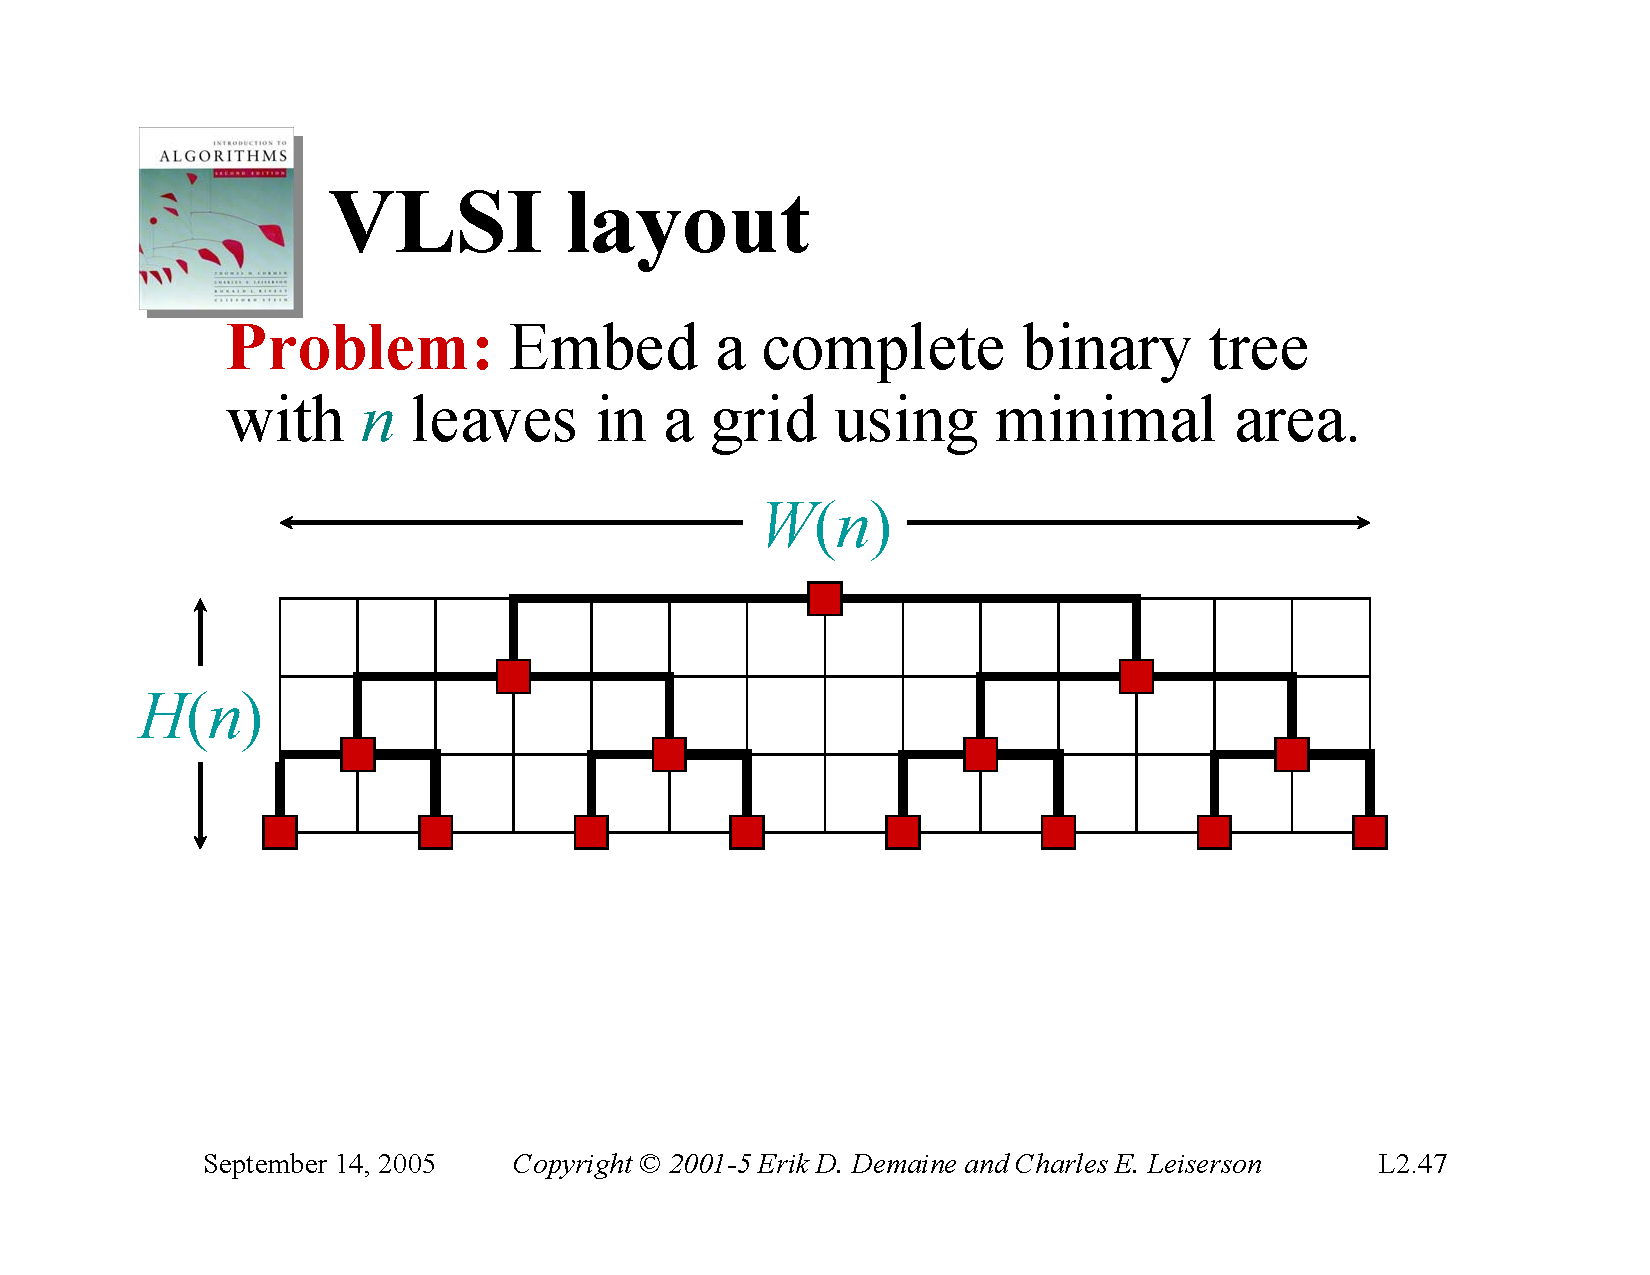
\includegraphics[width=\textwidth, trim={1cm 5cm 2cm 7cm}, clip]{pages/lec3_47}
    \begin{minipage}{0.48\textwidth}
        \pause
        \begin{equation*}
            \begin{split}
                H(n) =& H\left(\frac{n}{2}\right) + \Theta(1) \\
                    =& \Theta(\lg n)
            \end{split}
        \end{equation*}
    \end{minipage}
    \hfill
    \begin{minipage}{0.48\textwidth}
        \pause
        \begin{equation*}
            \begin{split}
                W(n) =& 2W\left(\frac{n}{2}\right) + \Theta(1) \\
                    =& \Theta(n)
            \end{split}
        \end{equation*}
    \end{minipage}
    \pause
    \begin{exampleblock}{ }
        \centering
        \Large
        \textbf{Area:} $ = \Theta(n \ln n)$
    \end{exampleblock}
\end{frame}

\begin{frame}{H-tree Embedding}
    \begin{minipage}{0.48\textwidth}
        \centering
        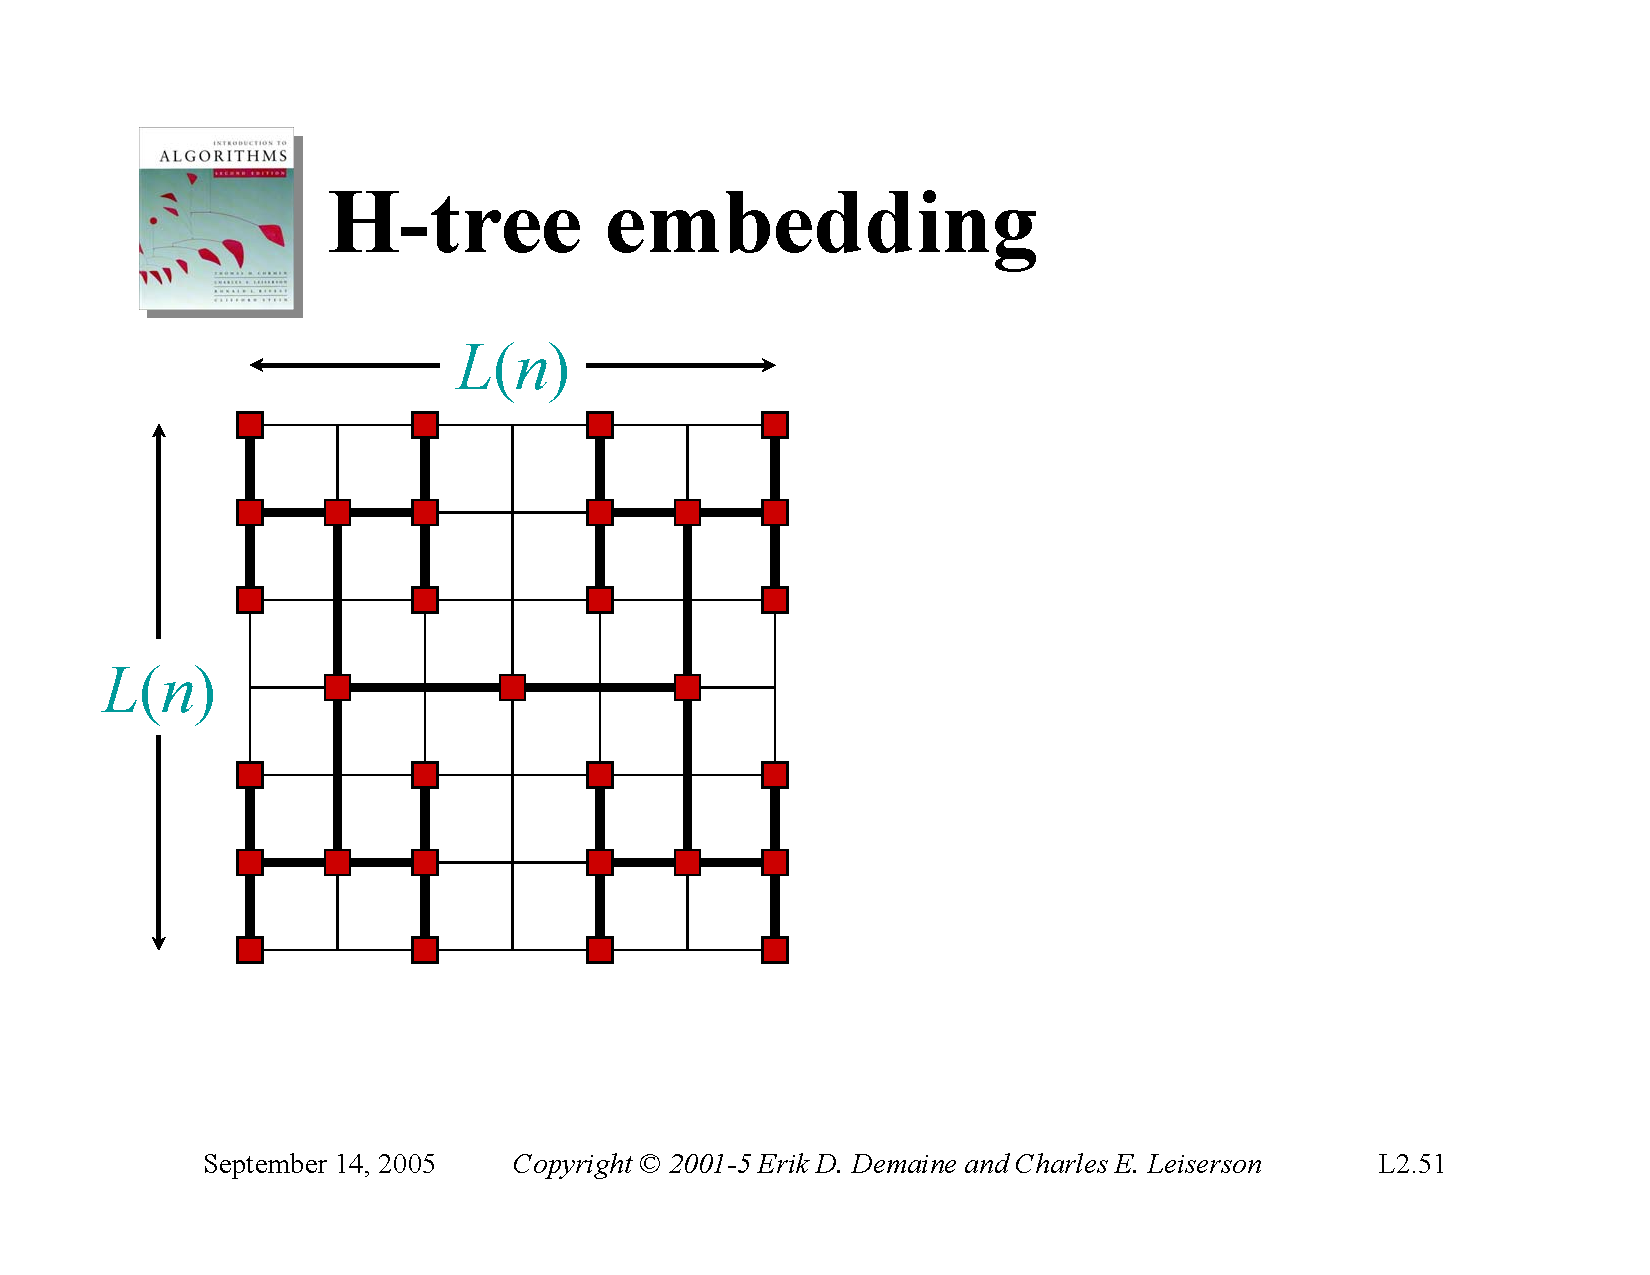
\includegraphics[width=\textwidth, trim={0.45cm 2.25cm 13.25cm 4.25cm}, clip]{pages/lec3_51}
    \end{minipage}
    \hfill
    \begin{minipage}{0.48\textwidth}
    \end{minipage}
\end{frame}

\begin{frame}{H-tree Embedding}
    \begin{minipage}{0.48\textwidth}
        \centering
        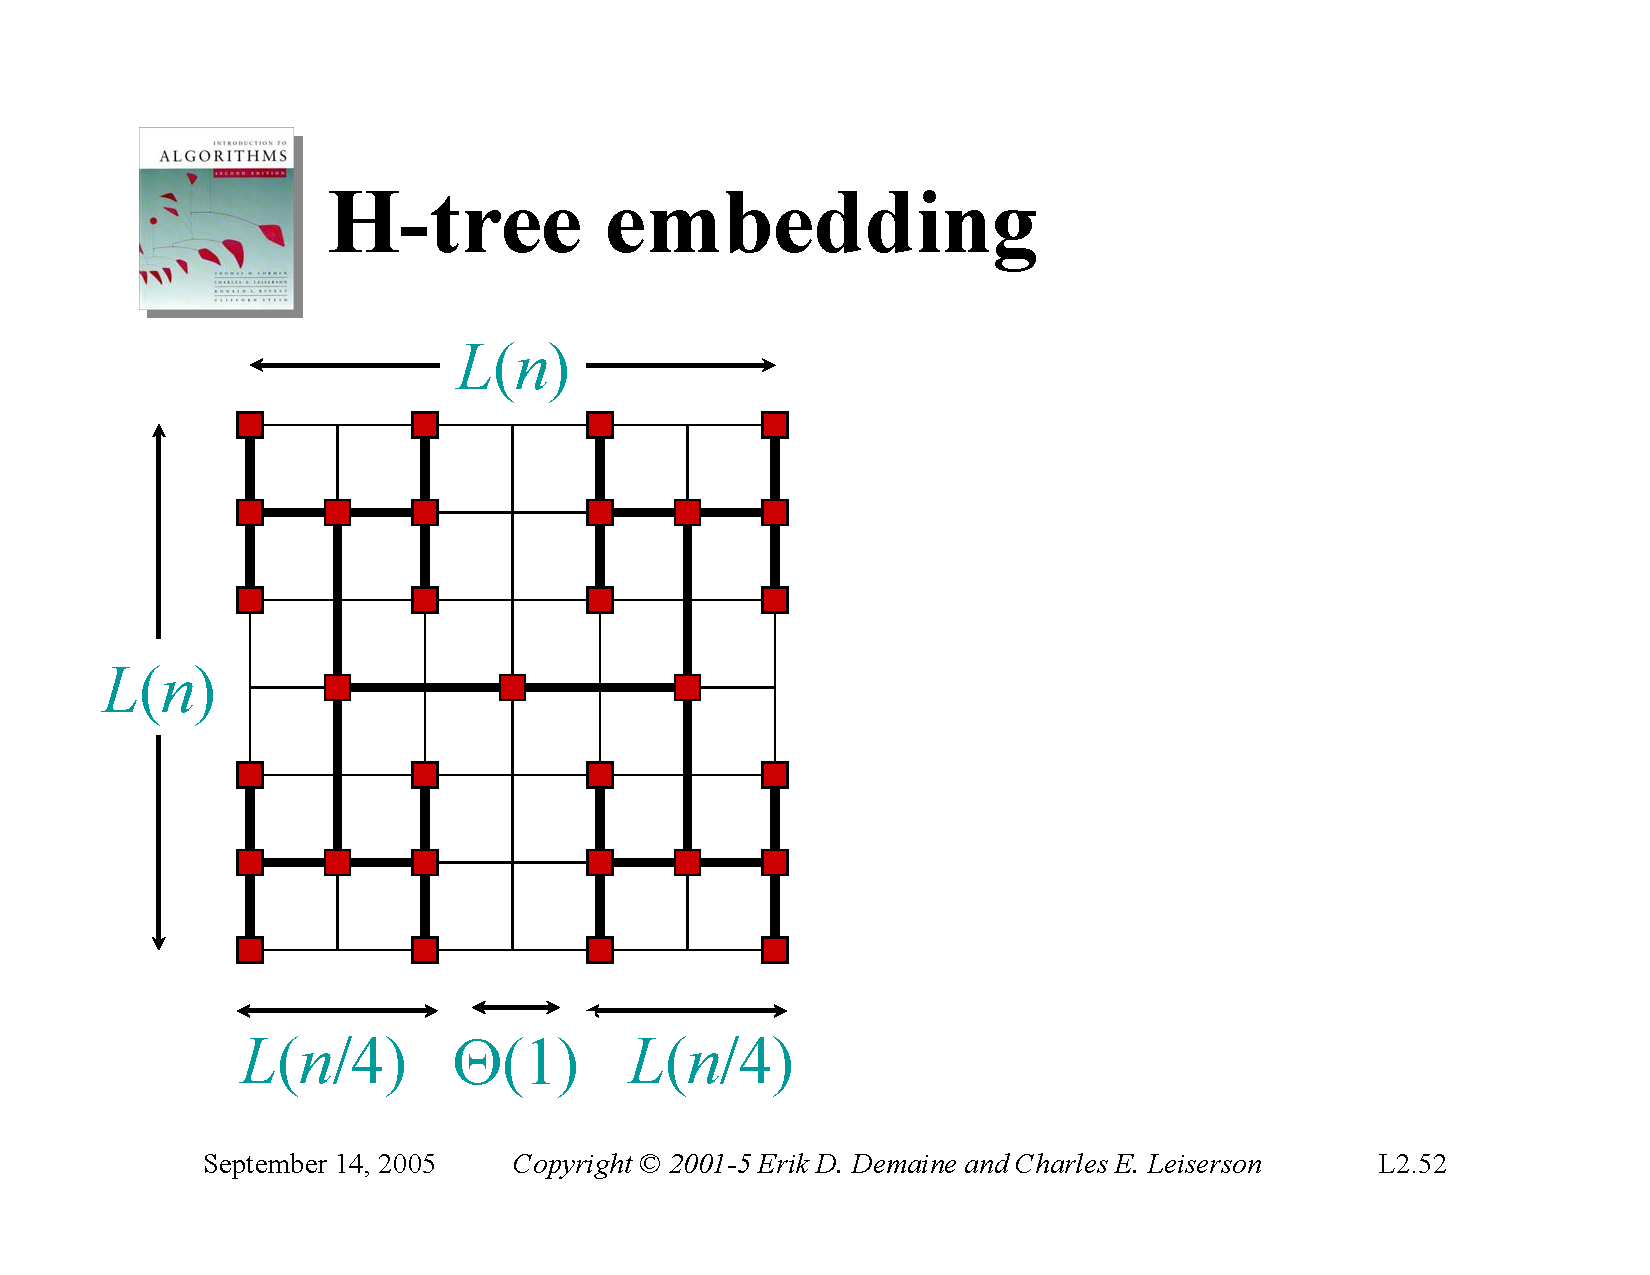
\includegraphics[width=\textwidth, trim={0.45cm 1.75cm 13.25cm 4.25cm}, clip]{pages/lec3_52}
    \end{minipage}
    \hfill
    \begin{minipage}{0.48\textwidth}
        \pause
        \centering
        \begin{equation*}
            \begin{split}
                L(n) =& 2L\left(\frac{n}{4} \right) + \Theta(1) \\
                     =& \Theta(\sqrt{n})
            \end{split}
        \end{equation*}
        \pause
        \Large
        \textbf{Area:} $ = \Theta(n)$
    \end{minipage}
\end{frame}

\begin{frame}{Conclusions}
    \begin{itemize}
        \item Divide and conquer is just one of several powerful techniques for algorithm design.
        \item Divide-and-conquer algorithms can be analyzed using recurrences and the master method (so practice this math).
        \item The divide-and-conquer strategy often leads to efficient algorithms.
    \end{itemize}
\end{frame}

\begin{frame}{}
    \centering
    \Huge End of Lecture 3.
\end{frame}

\section*{Takeaways}

% Tim Duncan's Top 5 Fundamental Takeaways of the Today's Class
\begin{frame}{TDT5FTOTTC}
    \centering
    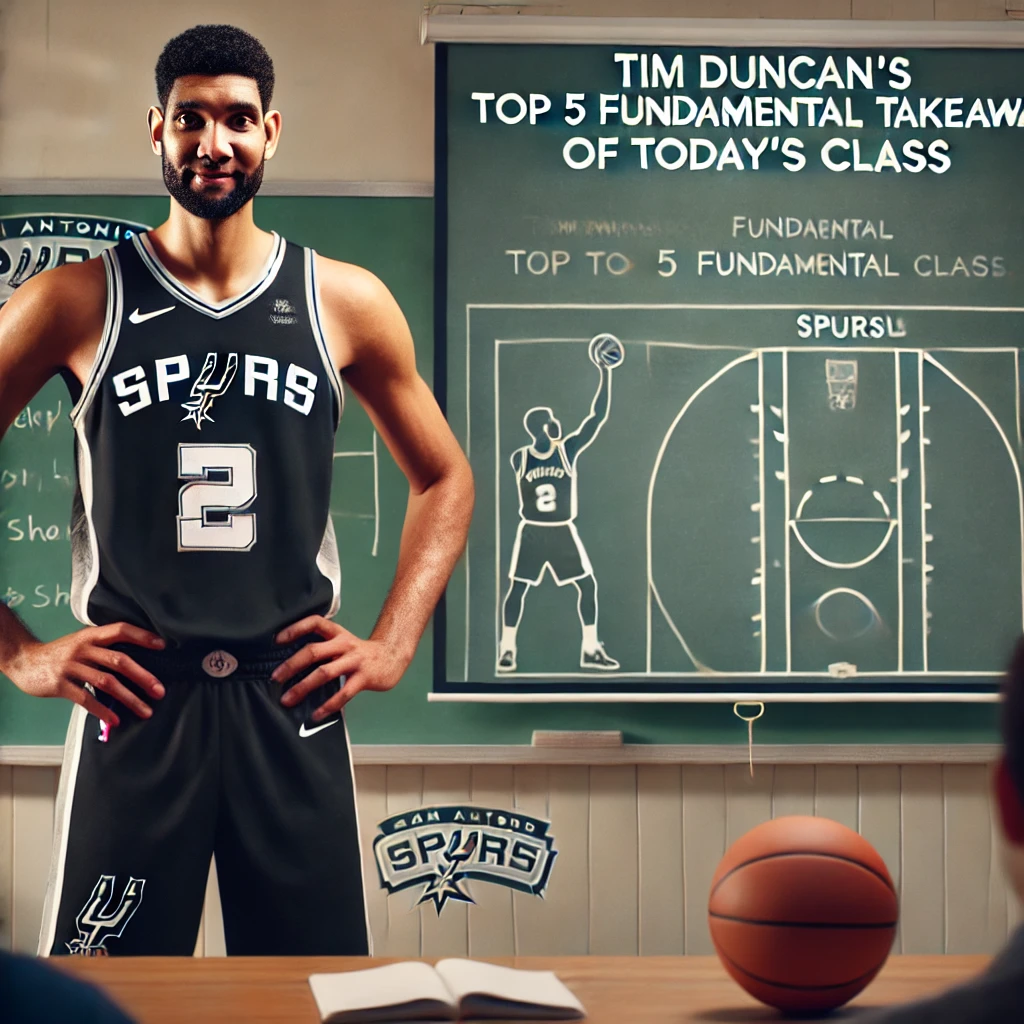
\includegraphics[width=0.75\textwidth]{figures/tim.png}
\end{frame}

\begin{frame}{Top 5 Fundamental Takeaways}
    \footnotesize
    \begin{enumerate} \pause
        \item[5] \textbf{Applications Beyond Sorting and Searching}: Techniques like VLSI tree layout and H-tree embedding optimize spatial and computational complexity in fields like circuit design and geometry. \pause

        \item[4] \textbf{Optimized Computation Techniques}: Problems such as exponentiation ($O(\log n)$) and Fibonacci computation ($O(\log n)$) benefit from divide-and-conquer methods that replace naive exponential-time approaches. \pause

        \item[3] \textbf{Master Theorem for Complexity Analysis}: A formulaic method to determine the time complexity of divide-and-conquer algorithms based on recurrence relations. \pause

        \item[2] \textbf{Efficient Algorithms Using Divide and Conquer}: Algorithms like merge sort ($O(n \log n)$), binary search ($O(\log n)$), and Strassen’s matrix multiplication ($O(n^{2.81})$) leverage this paradigm for improved efficiency. \pause

        \item[1] \textbf{Divide and Conquer Paradigm}: This algorithmic approach breaks a problem into smaller subproblems, solves them recursively, and combines the results efficiently. \pause

    \end{enumerate}
\end{frame}

\begin{frame}{Introduction to Algorithms}
    \centering
    
\includegraphics[width=0.45\textwidth]{figures/book_cover.jpg} \\
    \vspace{5mm}{
        \tiny
        Content has been extracted from \textit{Introduction to Algorithms}, Fourth Edition, by Cormen, Leiserson, Rivest, and Stein. MIT Press. 2022.\\
        Visit \url{https://mitpress.mit.edu/9780262046305/introduction-to-algorithms/}.\\
        Original slides from \textit{Introduction to Algorithms 6.046J/18.401J}, Fall 2005 Class by Prof. Charles Leiserson and Prof. Erik Demaine. MIT OpenCourseWare Initiative available at \url{https://ocw.mit.edu/courses/6-046j-introduction-to-algorithms-sma-5503-fall-2005/}.\\
    }
\end{frame}

\end{document}
